\documentclass[12pt, a4paper]{article}

\newcommand{\kafedra}{ИИТ} % Кафедра X

\newcommand{\numberOfLab}{2} % Лабораторная работа №X
\newcommand{\semestr}{2} % За X семестр
\newcommand{\distiplina}{ОАиП} % По дисциплине <<X>>
\newcommand{\labTitle}{Структуры, перечисления, объединения} % Тема: <<X>>

% Выполнил
\newcommand{\kurs}{1} % Студент X курса
\newcommand{\group}{ПО-4 (1)} % группы X
\newcommand{\labAuthor}{Галанин П. И.} % X

% Проверил
\newcommand{\teacherStatus}{ст. преподаватель} % X
\newcommand{\teacher}{Хацкевич М. В.} % X

\newcommand{\labDate}{Брест, 2020} % X

\usepackage{../../sty/encoding} % кодировка
\usepackage{../../sty/titlePage} % титульный лист
\usepackage{../../sty/fields} % поля
\usepackage{../../sty/imgs} % картинки
\usepackage{../../sty/code} % исходный код
\usepackage{../../sty/labData} % для лабораторной

\begin{document}

% титульный лист
\maketitle
\setcounter{page}{2}

% содержание
\renewcommand{\contentsname}{Содержание}
\tableofcontents
\newpage

% контент
\labheading

\labgoal{Изучить синтаксис и правила работы со структурами. Реализовать программу с применением структур, перечислений и объединений.}

\labreport

\section{Условие}

Создать тип структуры согласно варинту, организовать поля этой структуры так, чтобы они содержали объединение, перечисление (можно добавить дополнительные поля) и битовое поле.

Создать массив структур, содержащий информацию согласно варианту индивидуального задания.

Реализовать работу с массивом структур через меню: ввод данных в массив, вывод собержимого массива на экран, сортировка по одному полю, удаления записи по заданному значению поля, выборка записей согласно индивидуального задания.

\begin{center}
    \textbf{Вариант 13}
\end{center}

Сведения об автомобиле состоят из номера, марки, фамилии владельца, признака прохождения техосмотра. Для каждой марки подсчитать количество автомобилей этой марки.

\section{Проект}

\subsection{Структура проекта}

\begin{verbatim}
.
├── Makefile
├── inc
│   ├── clearConsole.h
│   ├── del_data.h
│   ├── encoding.h
│   ├── getch.h
│   ├── input_data.h
│   ├── lab.h
│   ├── main.h
│   ├── menu.h
│   ├── out_data.h
│   ├── pause_console.h
│   └── sort_data
│       ├── sort_data.h
│       ├── sort_data_by_mark_field.h
│       ├── sort_data_by_osmotr_field.h
│       ├── sort_data_by_surname_field.h
│       └── sort_data_in_number_field.h
└── src
    ├── clearConsole.c
    ├── del_data.c
    ├── encoding.c
    ├── getch.c
    ├── input_data.c
    ├── lab.c
    ├── main.c
    ├── menu.c
    ├── out_data.c
    ├── pause_console.c
    └── sort_data
        ├── sort_data.c
        ├── sort_data_by_mark_field.c
        ├── sort_data_by_osmotr_field.c
        ├── sort_data_by_surname_field.c
        └── sort_data_in_number_field.c

4 directories, 31 files
\end{verbatim}

\subsection{Исходный код}

\subsubsection{Makefile}
\lstinputlisting[language=make]{13/Makefile}

\subsubsection{main()}
Блок-схема на рисунке \ref{fig:main}.
\lstinputlisting[language=C]{13/inc/main.h}
\lstinputlisting[language=C]{13/src/main.c}

\subsubsection{encoding()}
Блок-схема на рисунке \ref{fig:encoding}.
\lstinputlisting[language=C]{13/inc/encoding.h}
\lstinputlisting[language=C]{13/src/encoding.c}

\subsubsection{lab()}
Блок-схема на рисунке \ref{fig:lab}.
\lstinputlisting[language=C]{13/inc/lab.h}
\lstinputlisting[language=C]{13/src/lab.c}

\subsubsection{clearConsole()}
Блок-схема на рисунке \ref{fig:clear_console}.
\lstinputlisting[language=C]{13/inc/clearConsole.h}
\lstinputlisting[language=C]{13/src/clearConsole.c}

\subsubsection{getch()}
\lstinputlisting[language=C]{13/inc/getch.h}
\lstinputlisting[language=C]{13/src/getch.c}

\subsubsection{pause\_console()}
\lstinputlisting[language=C]{13/inc/pause_console.h}
\lstinputlisting[language=C]{13/src/pause_console.c}

\subsubsection{menu()}
Блок-схема на рисунке \ref{fig:menu}.
\lstinputlisting[language=C]{13/inc/menu.h}
\lstinputlisting[language=C]{13/src/menu.c}

\subsubsection{input\_data()}
Блок-схема на рисунке \ref{fig:input_data}.
\lstinputlisting[language=C]{13/inc/input_data.h}
\lstinputlisting[language=C]{13/src/input_data.c}

\subsubsection{out\_data()}
Блок-схема на рисунке \ref{fig:out_data}.
\lstinputlisting[language=C]{13/inc/out_data.h}
\lstinputlisting[language=C]{13/src/out_data.c}

\subsubsection{sort\_data/sort\_data()}
\lstinputlisting[language=C]{13/inc/sort_data/sort_data.h}
\lstinputlisting[language=C]{13/src/sort_data/sort_data.c}

\subsubsection{sort\_data/sort\_data\_in\_number\_field()}
\lstinputlisting[language=C]{13/inc/sort_data/sort_data_in_number_field.h}
\lstinputlisting[language=C]{13/src/sort_data/sort_data_in_number_field.c}

\subsubsection{sort\_data/sort\_data\_by\_mark\_field()}
\lstinputlisting[language=C]{13/inc/sort_data/sort_data_by_mark_field.h}
\lstinputlisting[language=C]{13/src/sort_data/sort_data_by_mark_field.c}

\subsubsection{sort\_data/sort\_data\_by\_surname\_field()}
\lstinputlisting[language=C]{13/inc/sort_data/sort_data_by_surname_field.h}
\lstinputlisting[language=C]{13/src/sort_data/sort_data_by_surname_field.c}

\subsubsection{sort\_data/sort\_data\_by\_osmotr\_field()}
\lstinputlisting[language=C]{13/inc/sort_data/sort_data_by_osmotr_field.h}
\lstinputlisting[language=C]{13/src/sort_data/sort_data_by_osmotr_field.c}

\subsubsection{del\_data()}
Блок-схема на рисунке \ref{fig:del_data}.
\lstinputlisting[language=C]{13/inc/del_data.h}
\lstinputlisting[language=C]{13/src/del_data.c}

\newpage

\section{Исполняемая программа}

Запускаю программу

\begin{tcolorbox}
\begin{verbatim}
Меню:
1. Ввод данных       
2. Вывод данных      
3. Сортирова по полю 
4. Удалить запись    
0. Выйти из программы
\end{verbatim}
\end{tcolorbox}

Выбираю пункт 1

\begin{tcolorbox}
\begin{verbatim}
Размер строки номера: 
\end{verbatim}
\end{tcolorbox}

Ввожу размер строки номера

\begin{tcolorbox}
\begin{verbatim}
Размер строки номера: 8  
Номер машины: 
\end{verbatim}
\end{tcolorbox}

Ввожу сам номер

\begin{tcolorbox}
\begin{verbatim}
Размер строки номера: 8  
Номер машины: fruf45

Размер строки марки машины: 
\end{verbatim}
\end{tcolorbox}

Ввожу размер строки марки 

\begin{tcolorbox}
\begin{verbatim}
Размер строки номера: 8
Номер машины: fruf45

Размер строки марки машины: 6
Марка машины: 
\end{verbatim}
\end{tcolorbox}

Ввожу марку машины

\begin{tcolorbox}
\begin{verbatim}
Размер строки номера: 8
Номер машины: fruf45

Размер строки марки машины: 6
Марка машины: БМВ

Размер строки фамилии владельца: 
\end{verbatim}
\end{tcolorbox}

Ввожу размер фамилии

\begin{tcolorbox}
\begin{verbatim}
Размер строки номера: 8
Номер машины: fruf45

Размер строки марки машины: 6
Марка машины: БМВ

Размер строки фамилии владельца: 10
Фамилия владельца:
\end{verbatim}
\end{tcolorbox}

Ввожу фамилию владельца

\begin{tcolorbox}
\begin{verbatim}
Размер строки номера: 8
Номер машины: fruf45

Размер строки марки машины: 6
Марка машины: БМВ

Размер строки фамилии владельца: 10
Фамилия владельца: Розетков

Осмотр: 
\end{verbatim}
\end{tcolorbox}

1 - прошел осмотр, 0 - не прошел просмотр, другая клавиша - ждет ввода

Открылось главное меню. Выбираю 2-ой пункт.

\begin{tcolorbox}
\begin{verbatim}
ID      Номер       Марка       Фамилия         Осмотр
0       fruf45      БМВ         Розетков        Пройден
Нажмите любую клавишу для продолжения...
\end{verbatim}
\end{tcolorbox}

Жму любую клавишу. Попадаю в главное меню. Выбираю пункт 1. Заполняю данные... Выбираю пункт 2 для просмотра.

\begin{tcolorbox}
\begin{verbatim}
ID      Номер       Марка       Фамилия         Осмотр
0       fruf45      БМВ         Розетков        Пройден
1       urt53f      Форд        Чемоданов       Не пройден
2       4fu55       Ауди        Зарядков        Пройден
3       5g54gd      Лада        Камеров         Не пройден
Нажмите любую клавишу для продолжения...   
\end{verbatim}
\end{tcolorbox}

Нажимаю любую клавишу. Попадаю в главное меню. Выбираю пункт 3.

\begin{tcolorbox}
\begin{verbatim}
1. Сортировка по номеру
2. Сортировка по марке  
3. Сортировка по фамилии
4. Сортировка по осмотру
0. Выйти

По какой строке сортировать: 
\end{verbatim}
\end{tcolorbox}

Выбираю пункт 1. Попадаю в главное меню. Нажимаю пункт 2 для вывода таблицы.

\begin{tcolorbox}
\begin{verbatim}
ID      Номер       Марка     Фамилия         Осмотр
0       4fu55       Ауди      Зарядков        Пройден
1       5g54gd      Лада      Камеров         Не пройден
2       fruf45      БМВ       Розетков        Пройден
3       urt53f      Форд      Чемоданов       Не пройден
Нажмите любую клавишу для продолжения...
\end{verbatim}
\end{tcolorbox}

Жму любую клавишу. Попадаю в главное меню. Выбираю пункт 3 для сортировки. Выбираю пункт 2. Попадаю в главное меню. Выбираю пункт 2 для вывода таблицы.

\begin{tcolorbox}
\begin{verbatim}
ID      Номер       Марка       Фамилия         Осмотр
0       4fu55       Ауди        Зарядков        Пройден
1       5g54gd      Лада        Камеров         Не пройден
2       fruf45      БМВ         Розетков        Пройден
3       urt53f      Форд        Чемоданов       Не пройден
Нажмите любую клавишу для продолжения...
\end{verbatim}
\end{tcolorbox}

Жму любую клавишу. Попадаю в главное меню. Выбираю пункт 3 для сортировки. Выбираю пункт 3. Попадаю в главное меню. Выбираю пункт 2 для вывода таблицы.

\begin{tcolorbox}
\begin{verbatim}
ID      Номер       Марка       Фамилия         Осмотр
0       4fu55       Ауди        Зарядков        Пройден
1       5g54gd      Лада        Камеров         Не пройден
2       fruf45      БМВ         Розетков        Пройден
3       urt53f      Форд        Чемоданов       Не пройден
Нажмите любую клавишу для продолжения...
\end{verbatim}
\end{tcolorbox}

Жму любую клавишу. Попадаю в главное меню. Выбираю пункт 3 для сортировки. Выбираю пункт 4. Попадаю в главное меню. Выбираю пункт 2 для вывода таблицы.

\begin{tcolorbox}
\begin{verbatim}
ID      Номер       Марка       Фамилия         Осмотр
0       4fu55       Ауди        Зарядков        Пройден   
1       fruf45      БМВ         Розетков        Пройден   
2       5g54gd      Лада        Камеров         Не пройден        
3       urt53f      Форд        Чемоданов       Не пройден
Нажмите любую клавишу для продолжения...
\end{verbatim}
\end{tcolorbox}

Жму любую клавишу. Попадаю в главное меню. Выбираю пункт 4 для удаления элемента.

\begin{tcolorbox}
\begin{verbatim}
Какой элемент удалить:
\end{verbatim}
\end{tcolorbox}

Жму 2. Жму Enter. Попадаю в главное меню. Выбираю пункт 2 для вывода таблицы.

\begin{tcolorbox}
\begin{verbatim}
ID      Номер       Марка       Фамилия         Осмотр
0       4fu55       Ауди        Зарядков        Пройден
1       fruf45      БМВ         Розетков        Пройден
2       urt53f      Форд        Чемоданов       Не пройден
Нажмите любую клавишу для продолжения...
\end{verbatim}
\end{tcolorbox}

Нажимаю любую клавишу. Переходу в главное меню. Выбираю пункт 4. Ввожу 55. Попадаю в главное меню. Выбираю пункт 2 для вывода таблицы.

\begin{tcolorbox}
\begin{verbatim}
ID      Номер       Марка       Фамилия         Осмотр
0       4fu55       Ауди        Зарядков        Пройден
1       fruf45      БМВ         Розетков        Пройден
2       urt53f      Форд        Чемоданов       Не пройден
Нажмите любую клавишу для продолжения...
\end{verbatim}
\end{tcolorbox}

Таблица не поменялась, так как нет такого ID.

Нажимаю 0, чтобы выйти из программы.

\labconclusion{}

\newpage

\section{Приложения}

\begin{figure}[h]
    \center{
        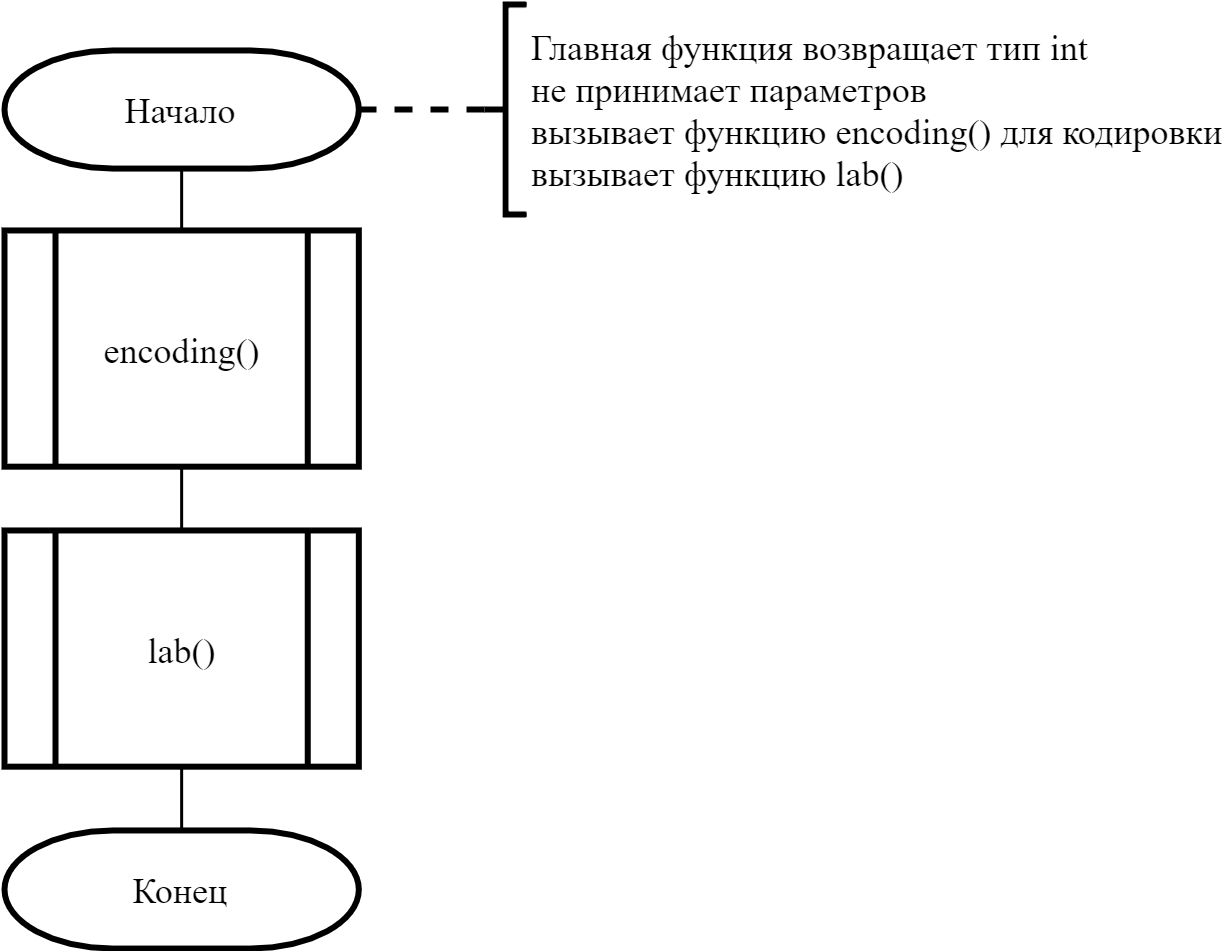
\includegraphics[]{13/flowcharts/main.png}
    }
    \caption{main()}
    \label{fig:main}
\end{figure}

\begin{figure}[h]
    \center{
        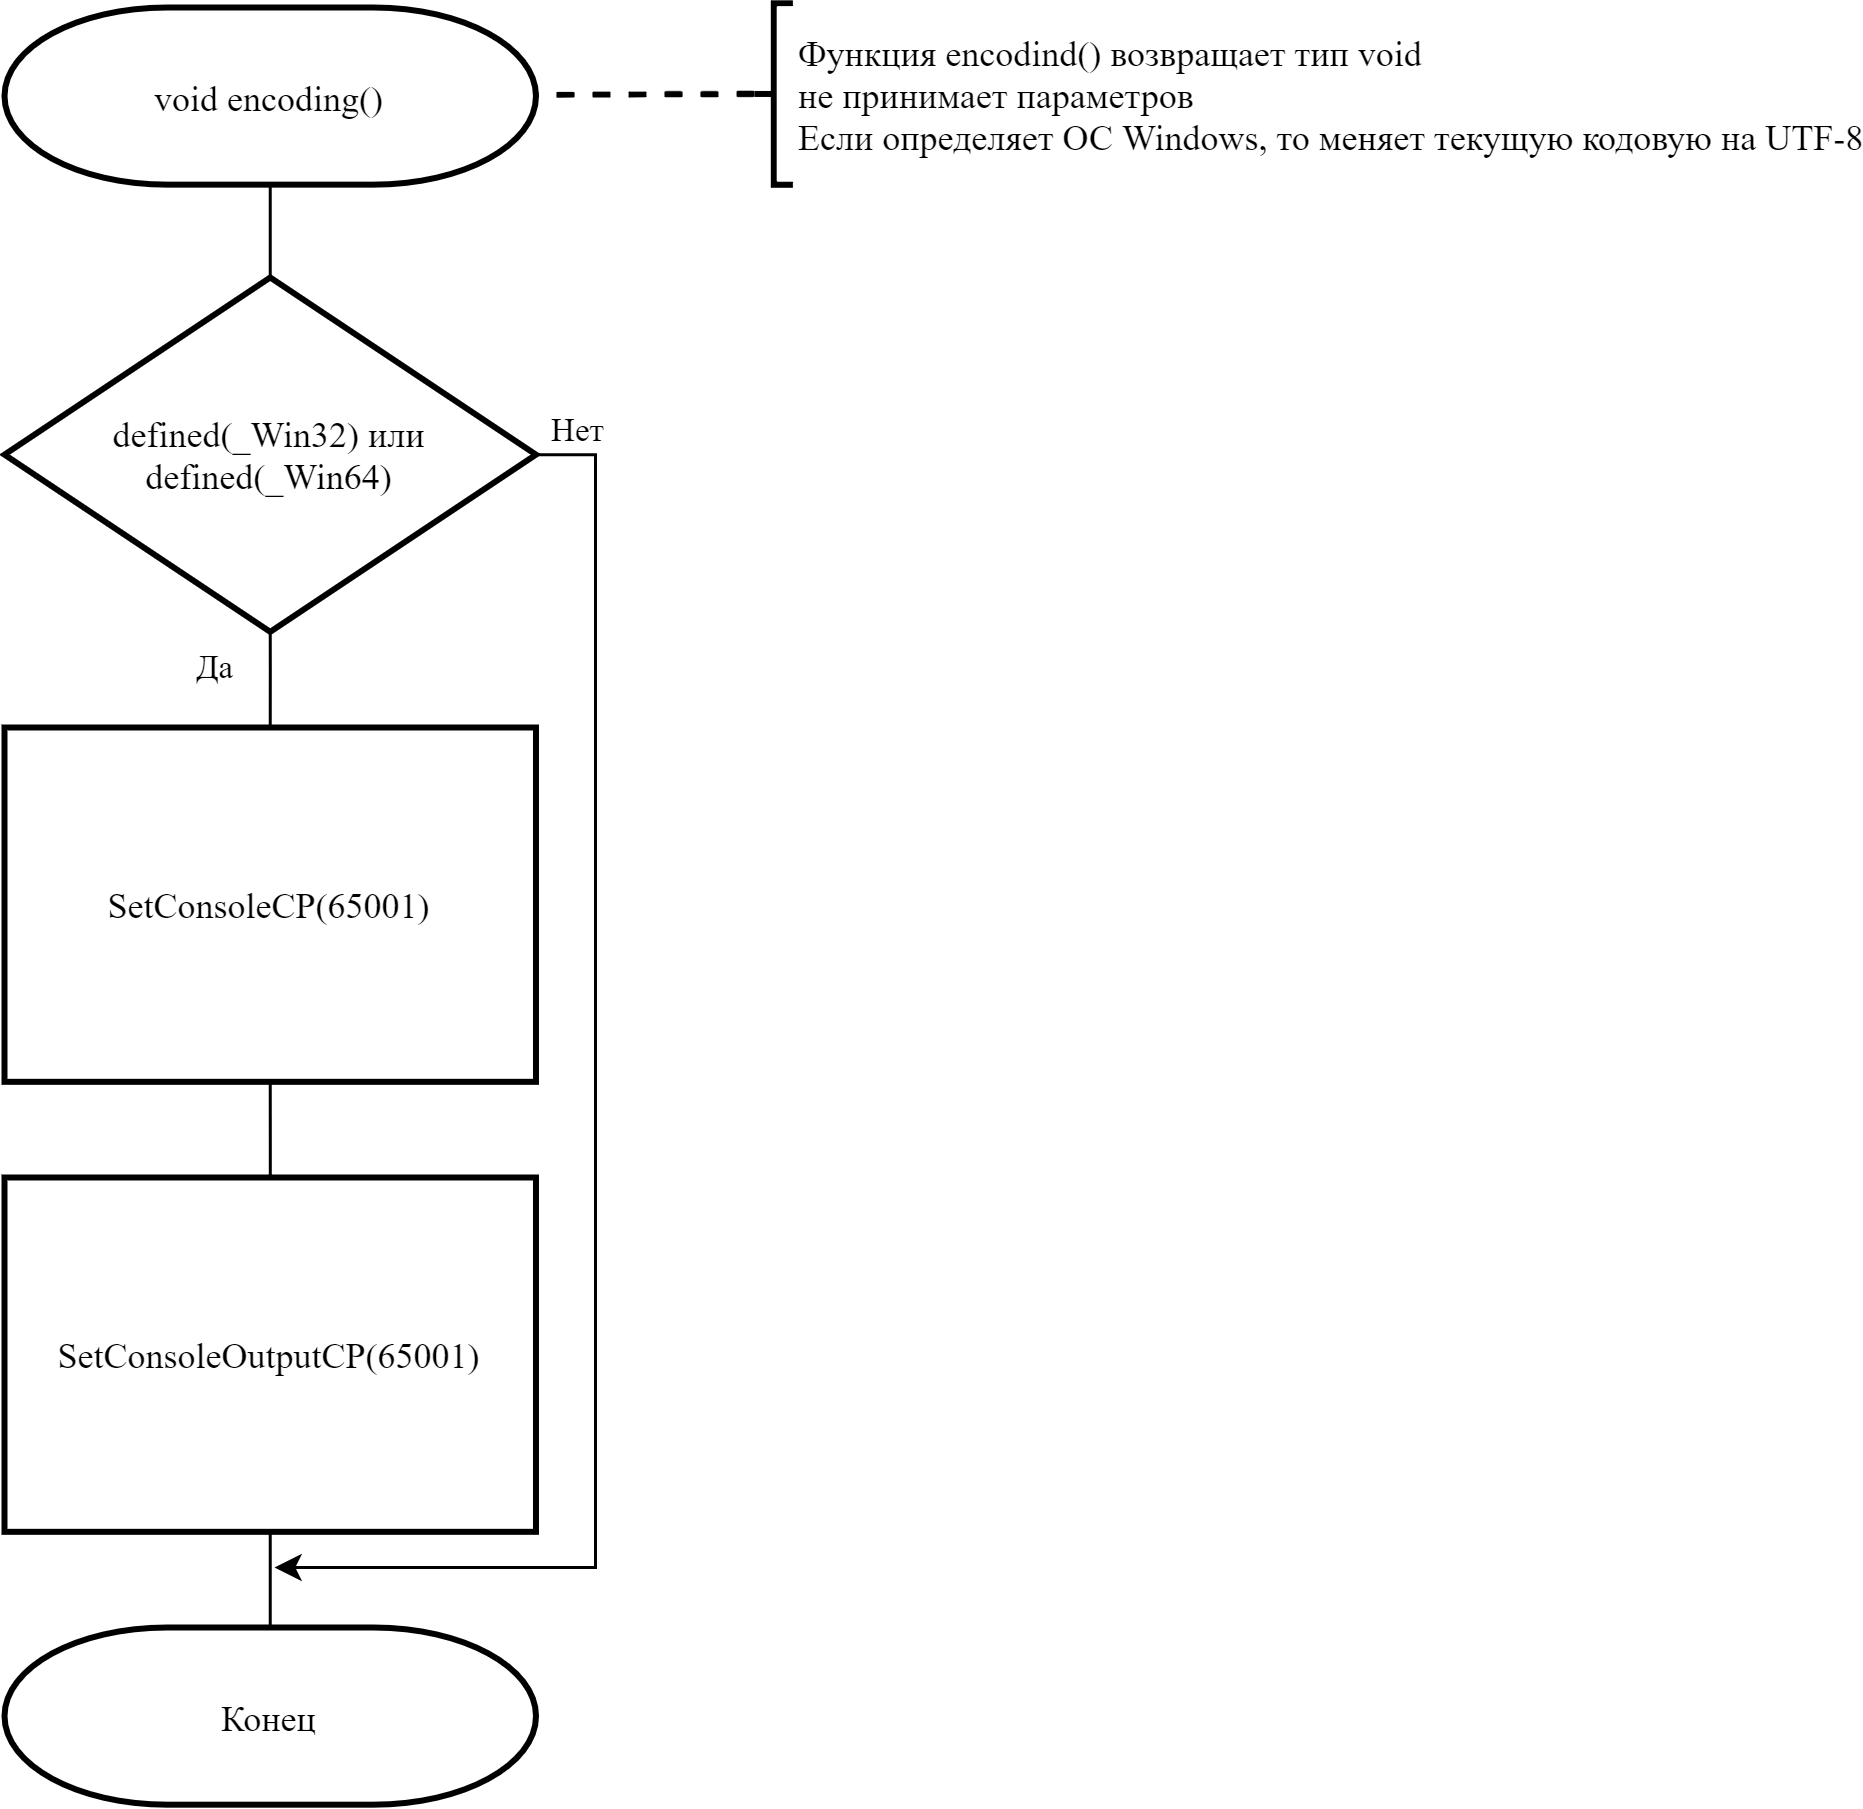
\includegraphics[]{13/flowcharts/encoding.png}
    }
    \caption{encoding()}
    \label{fig:encoding}
\end{figure}

\begin{figure}[h]
    \center{
        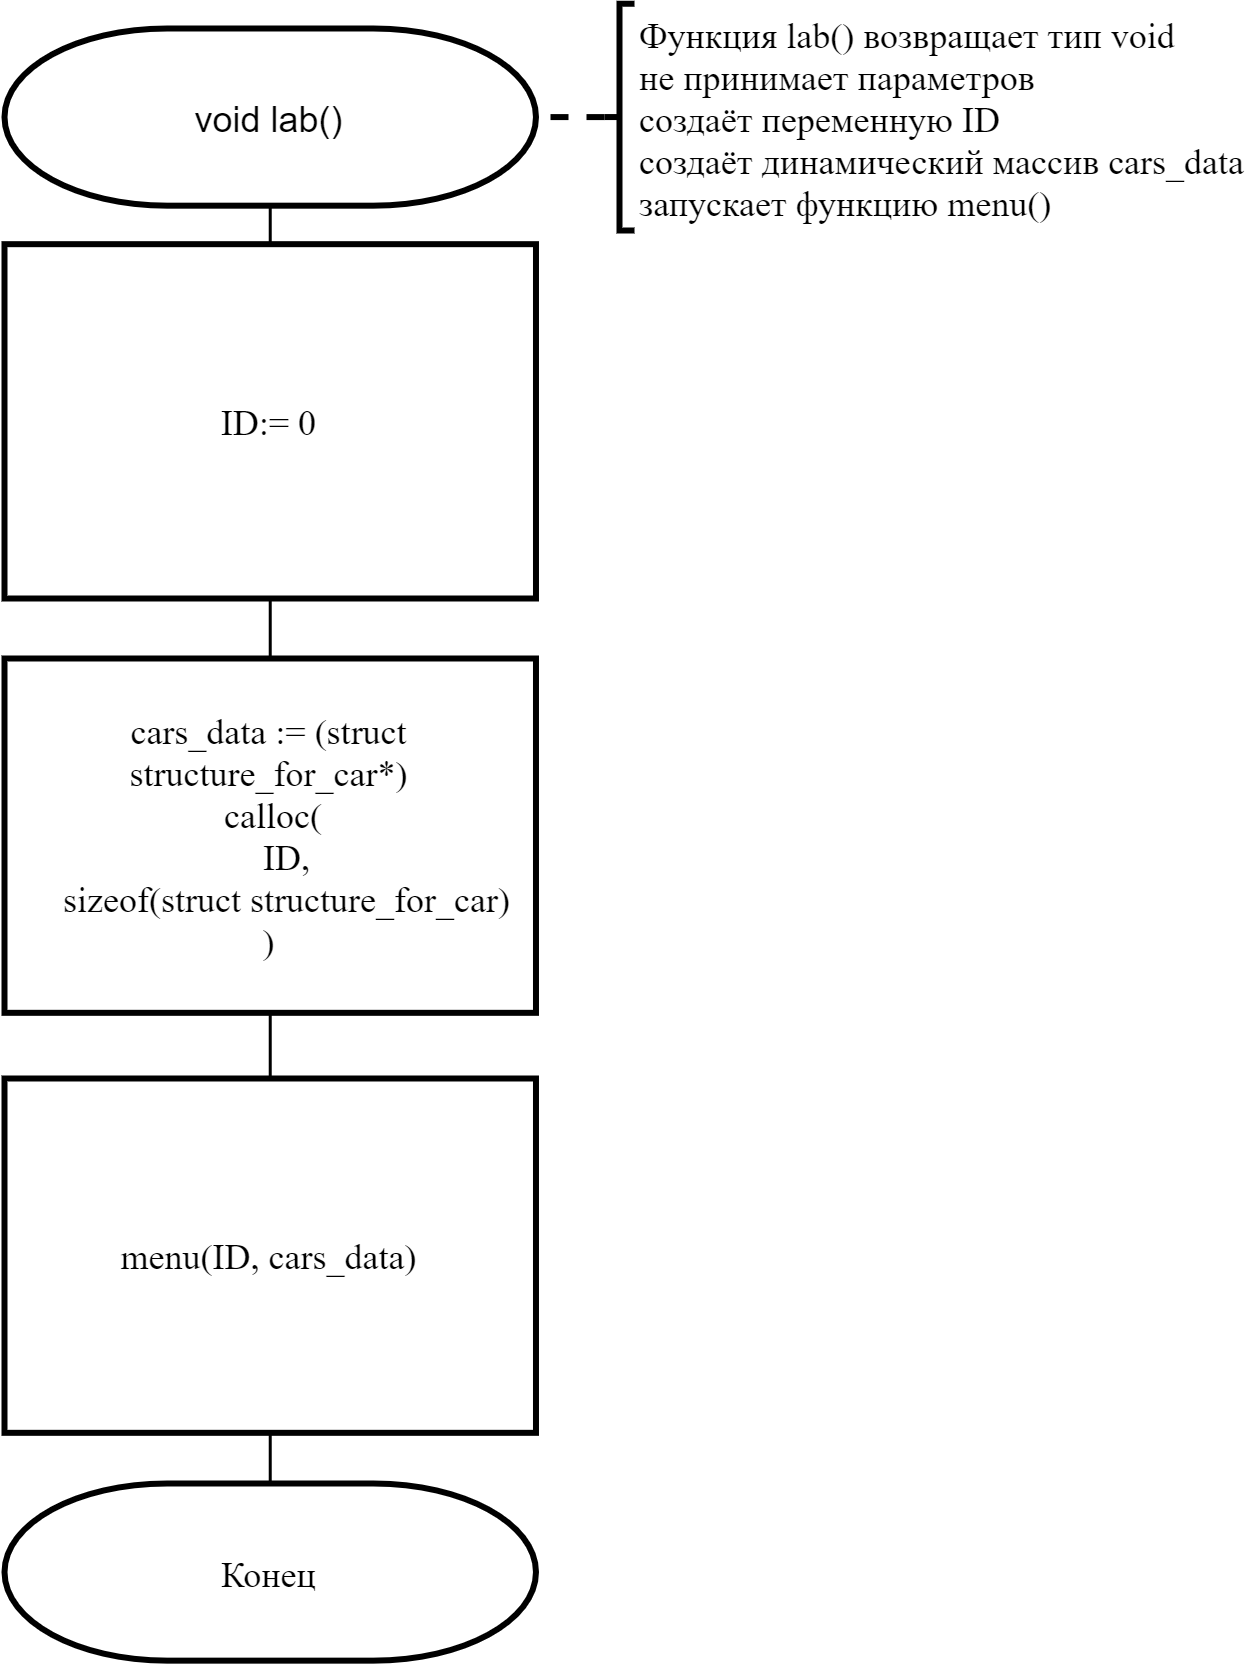
\includegraphics[]{13/flowcharts/lab.png}
    }
    \caption{lab()}
    \label{fig:lab}
\end{figure}

\begin{figure}[h]
    \center{
        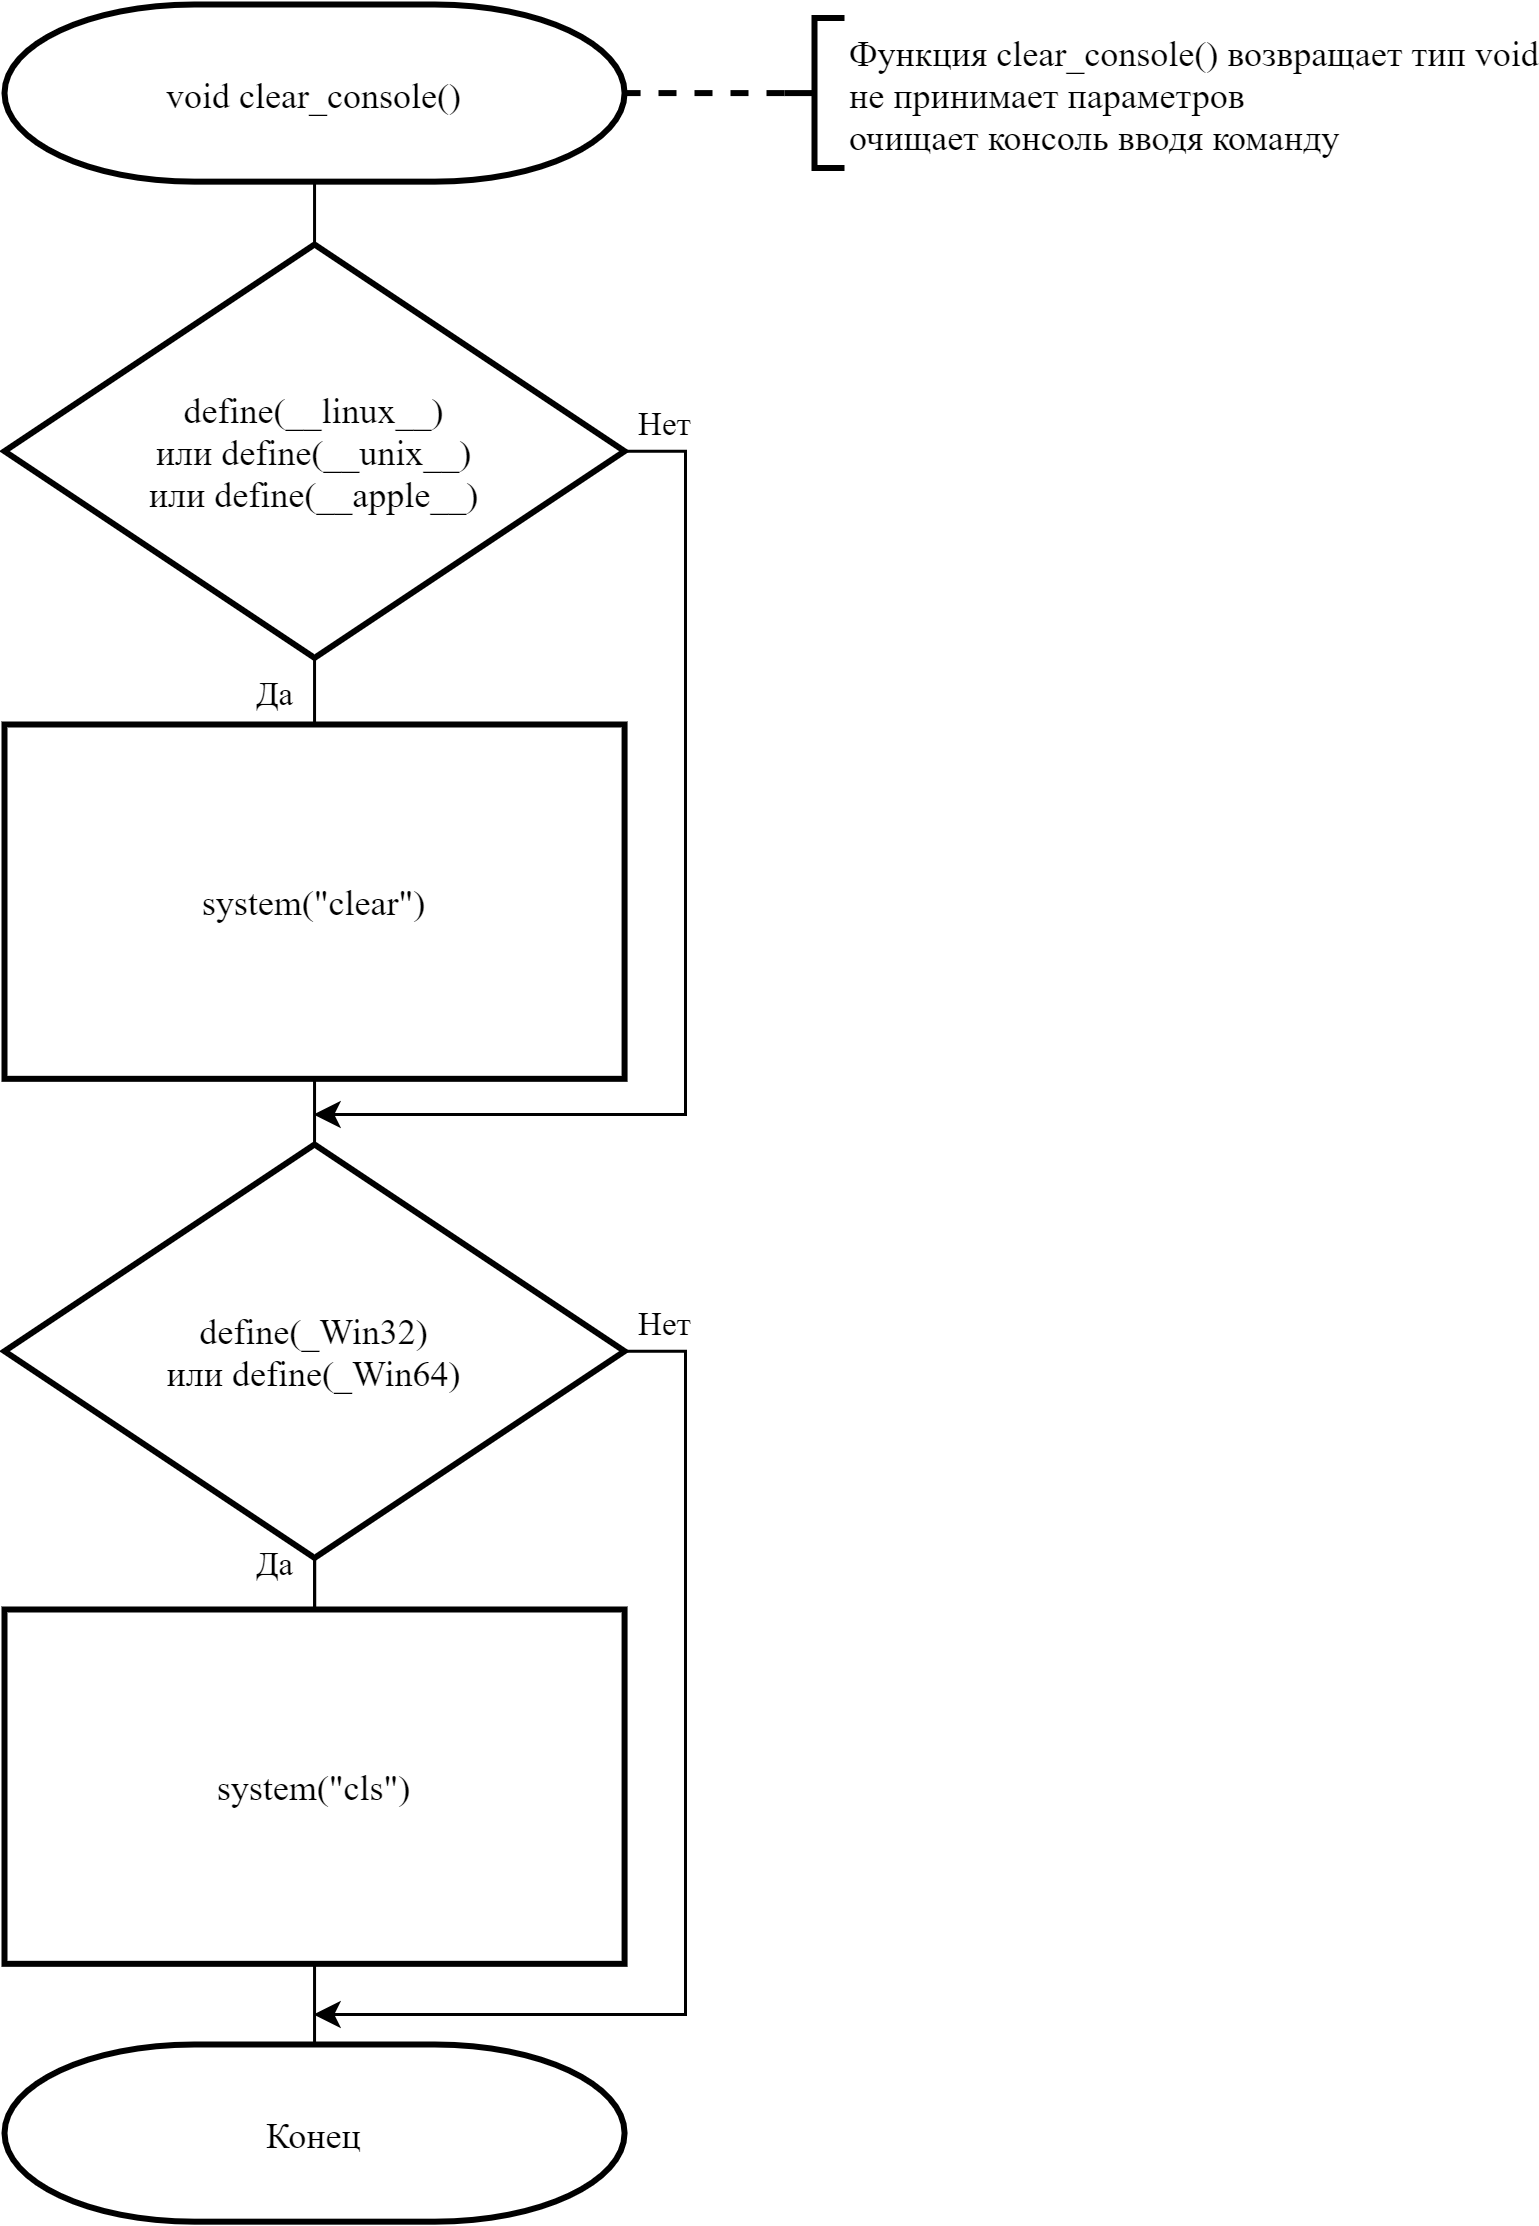
\includegraphics[]{13/flowcharts/clear_console.png}
    }
    \caption{clear\_console()}
    \label{fig:clear_console}
\end{figure}

\begin{figure}[h]
    \center{
        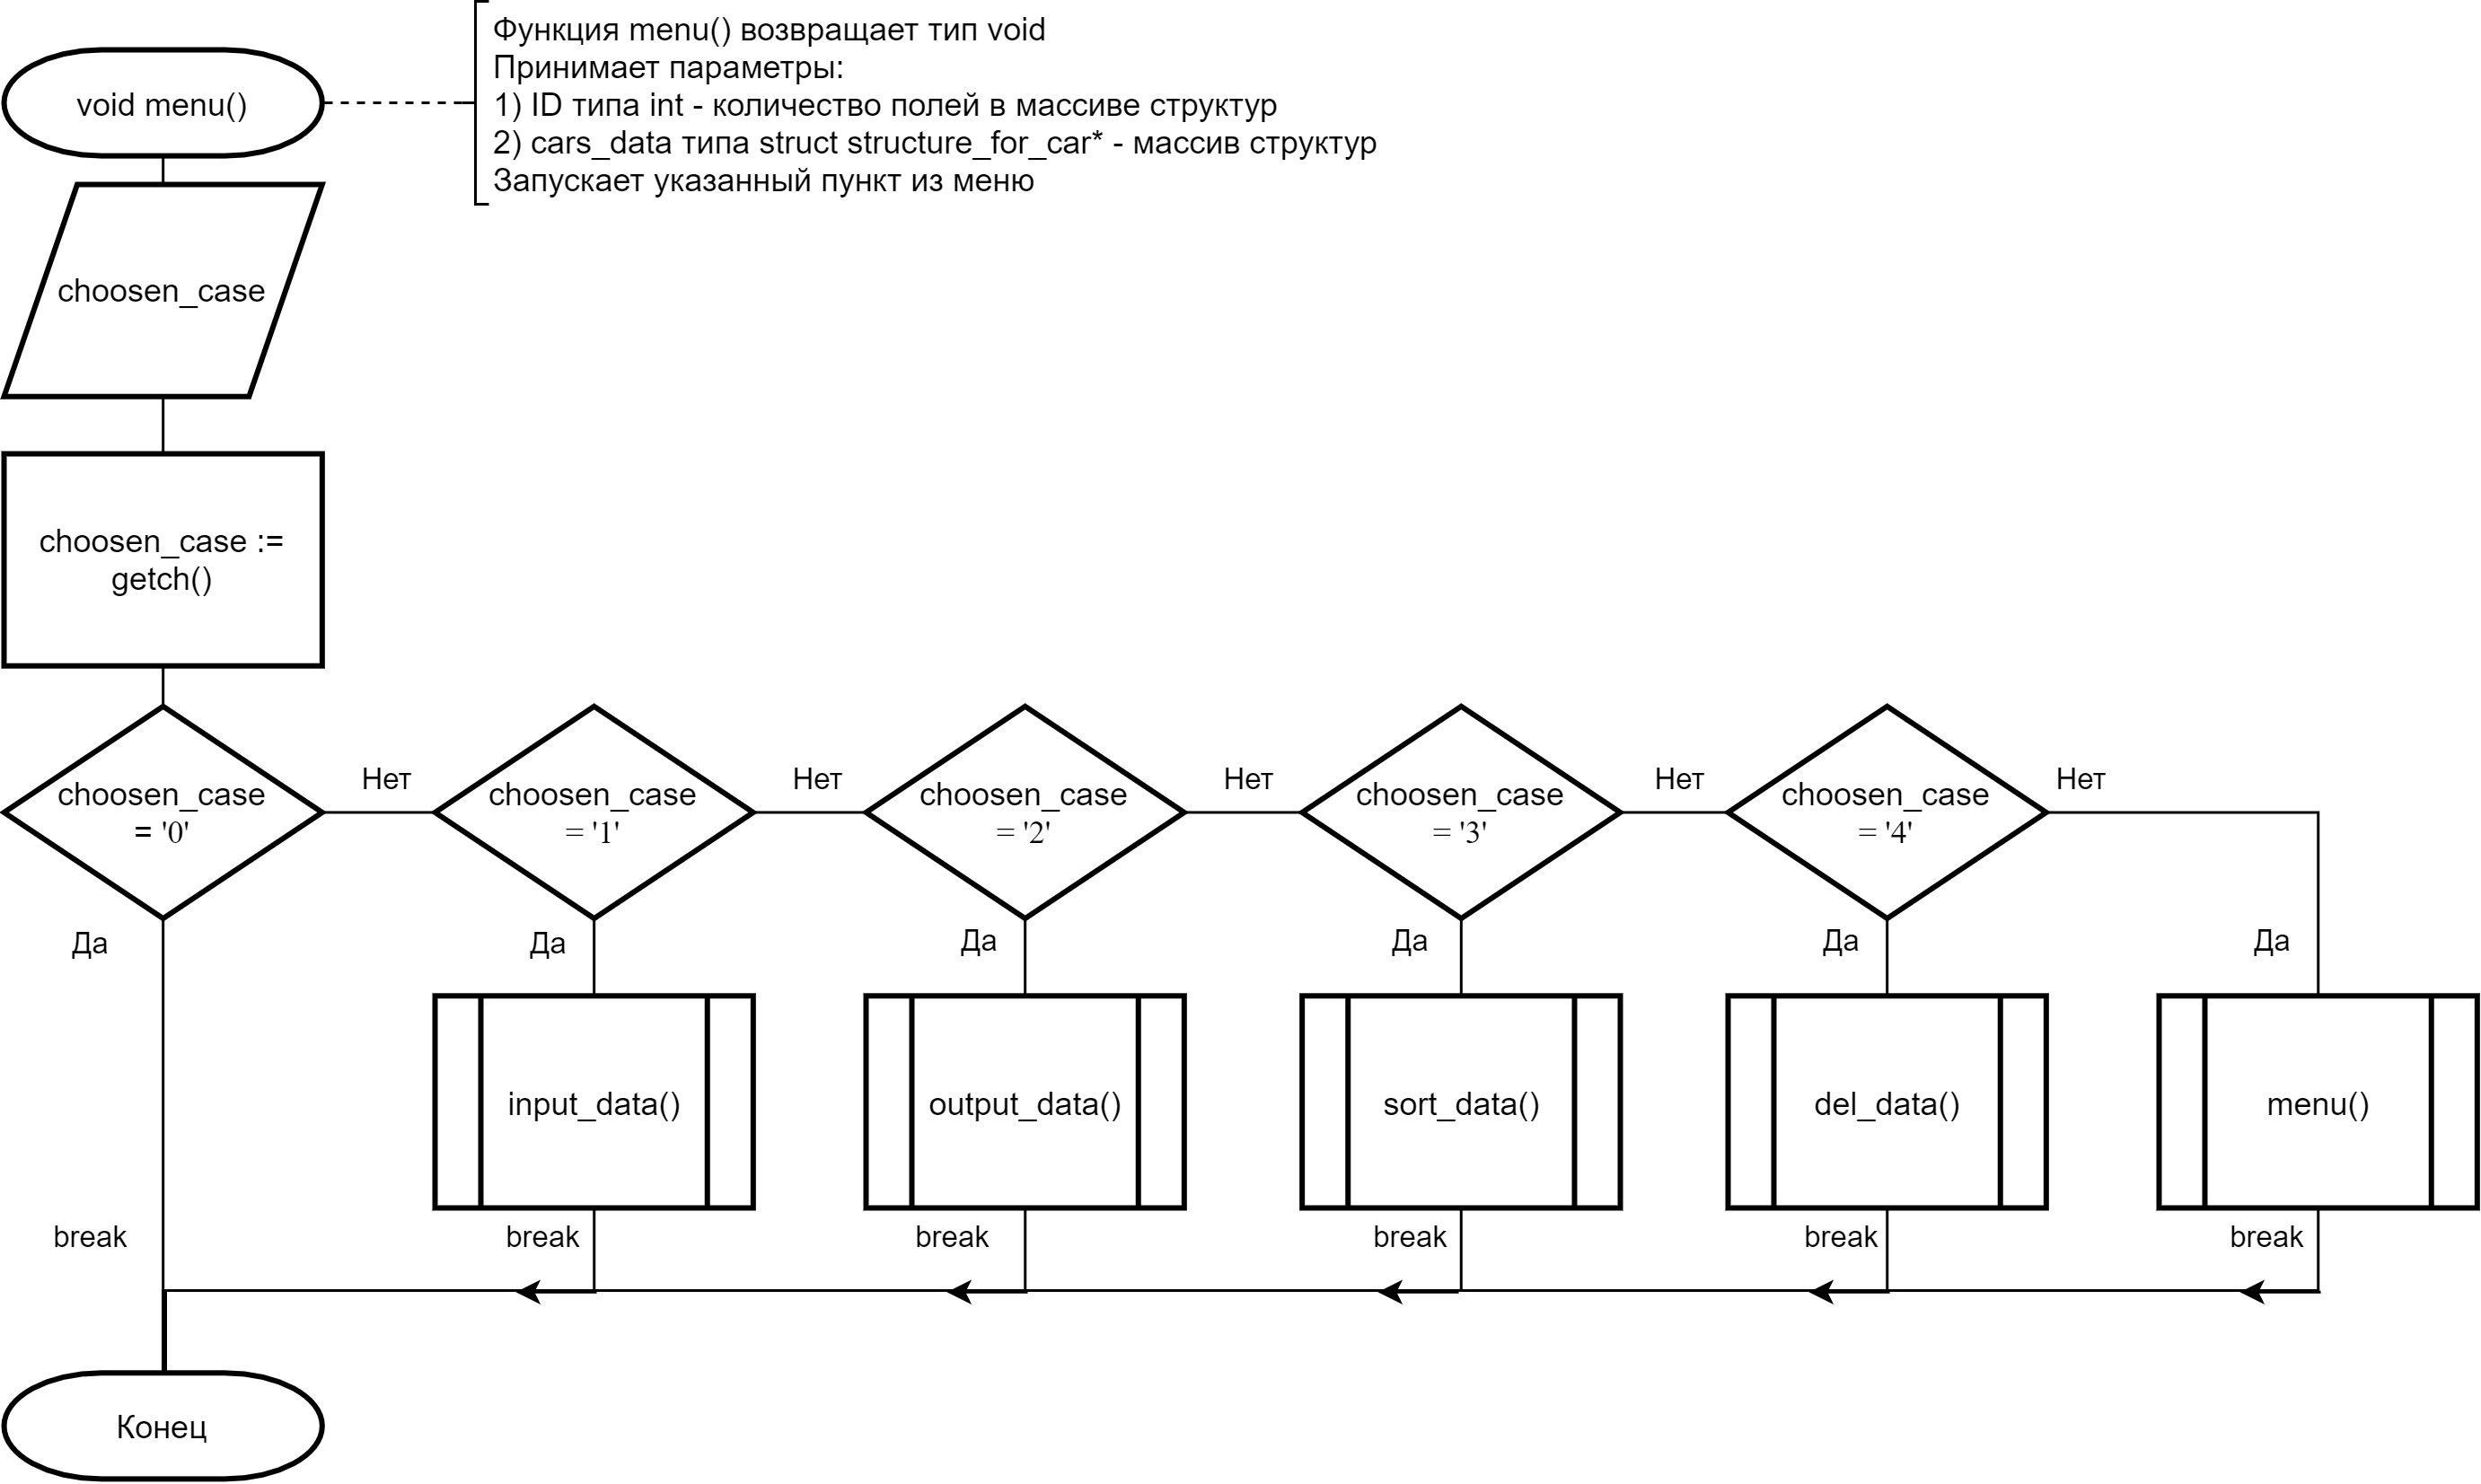
\includegraphics[width=16cm]{13/flowcharts/menu.png}
    }
    \caption{menu()}
    \label{fig:menu}
\end{figure}

\begin{figure}[h]
    \center{
        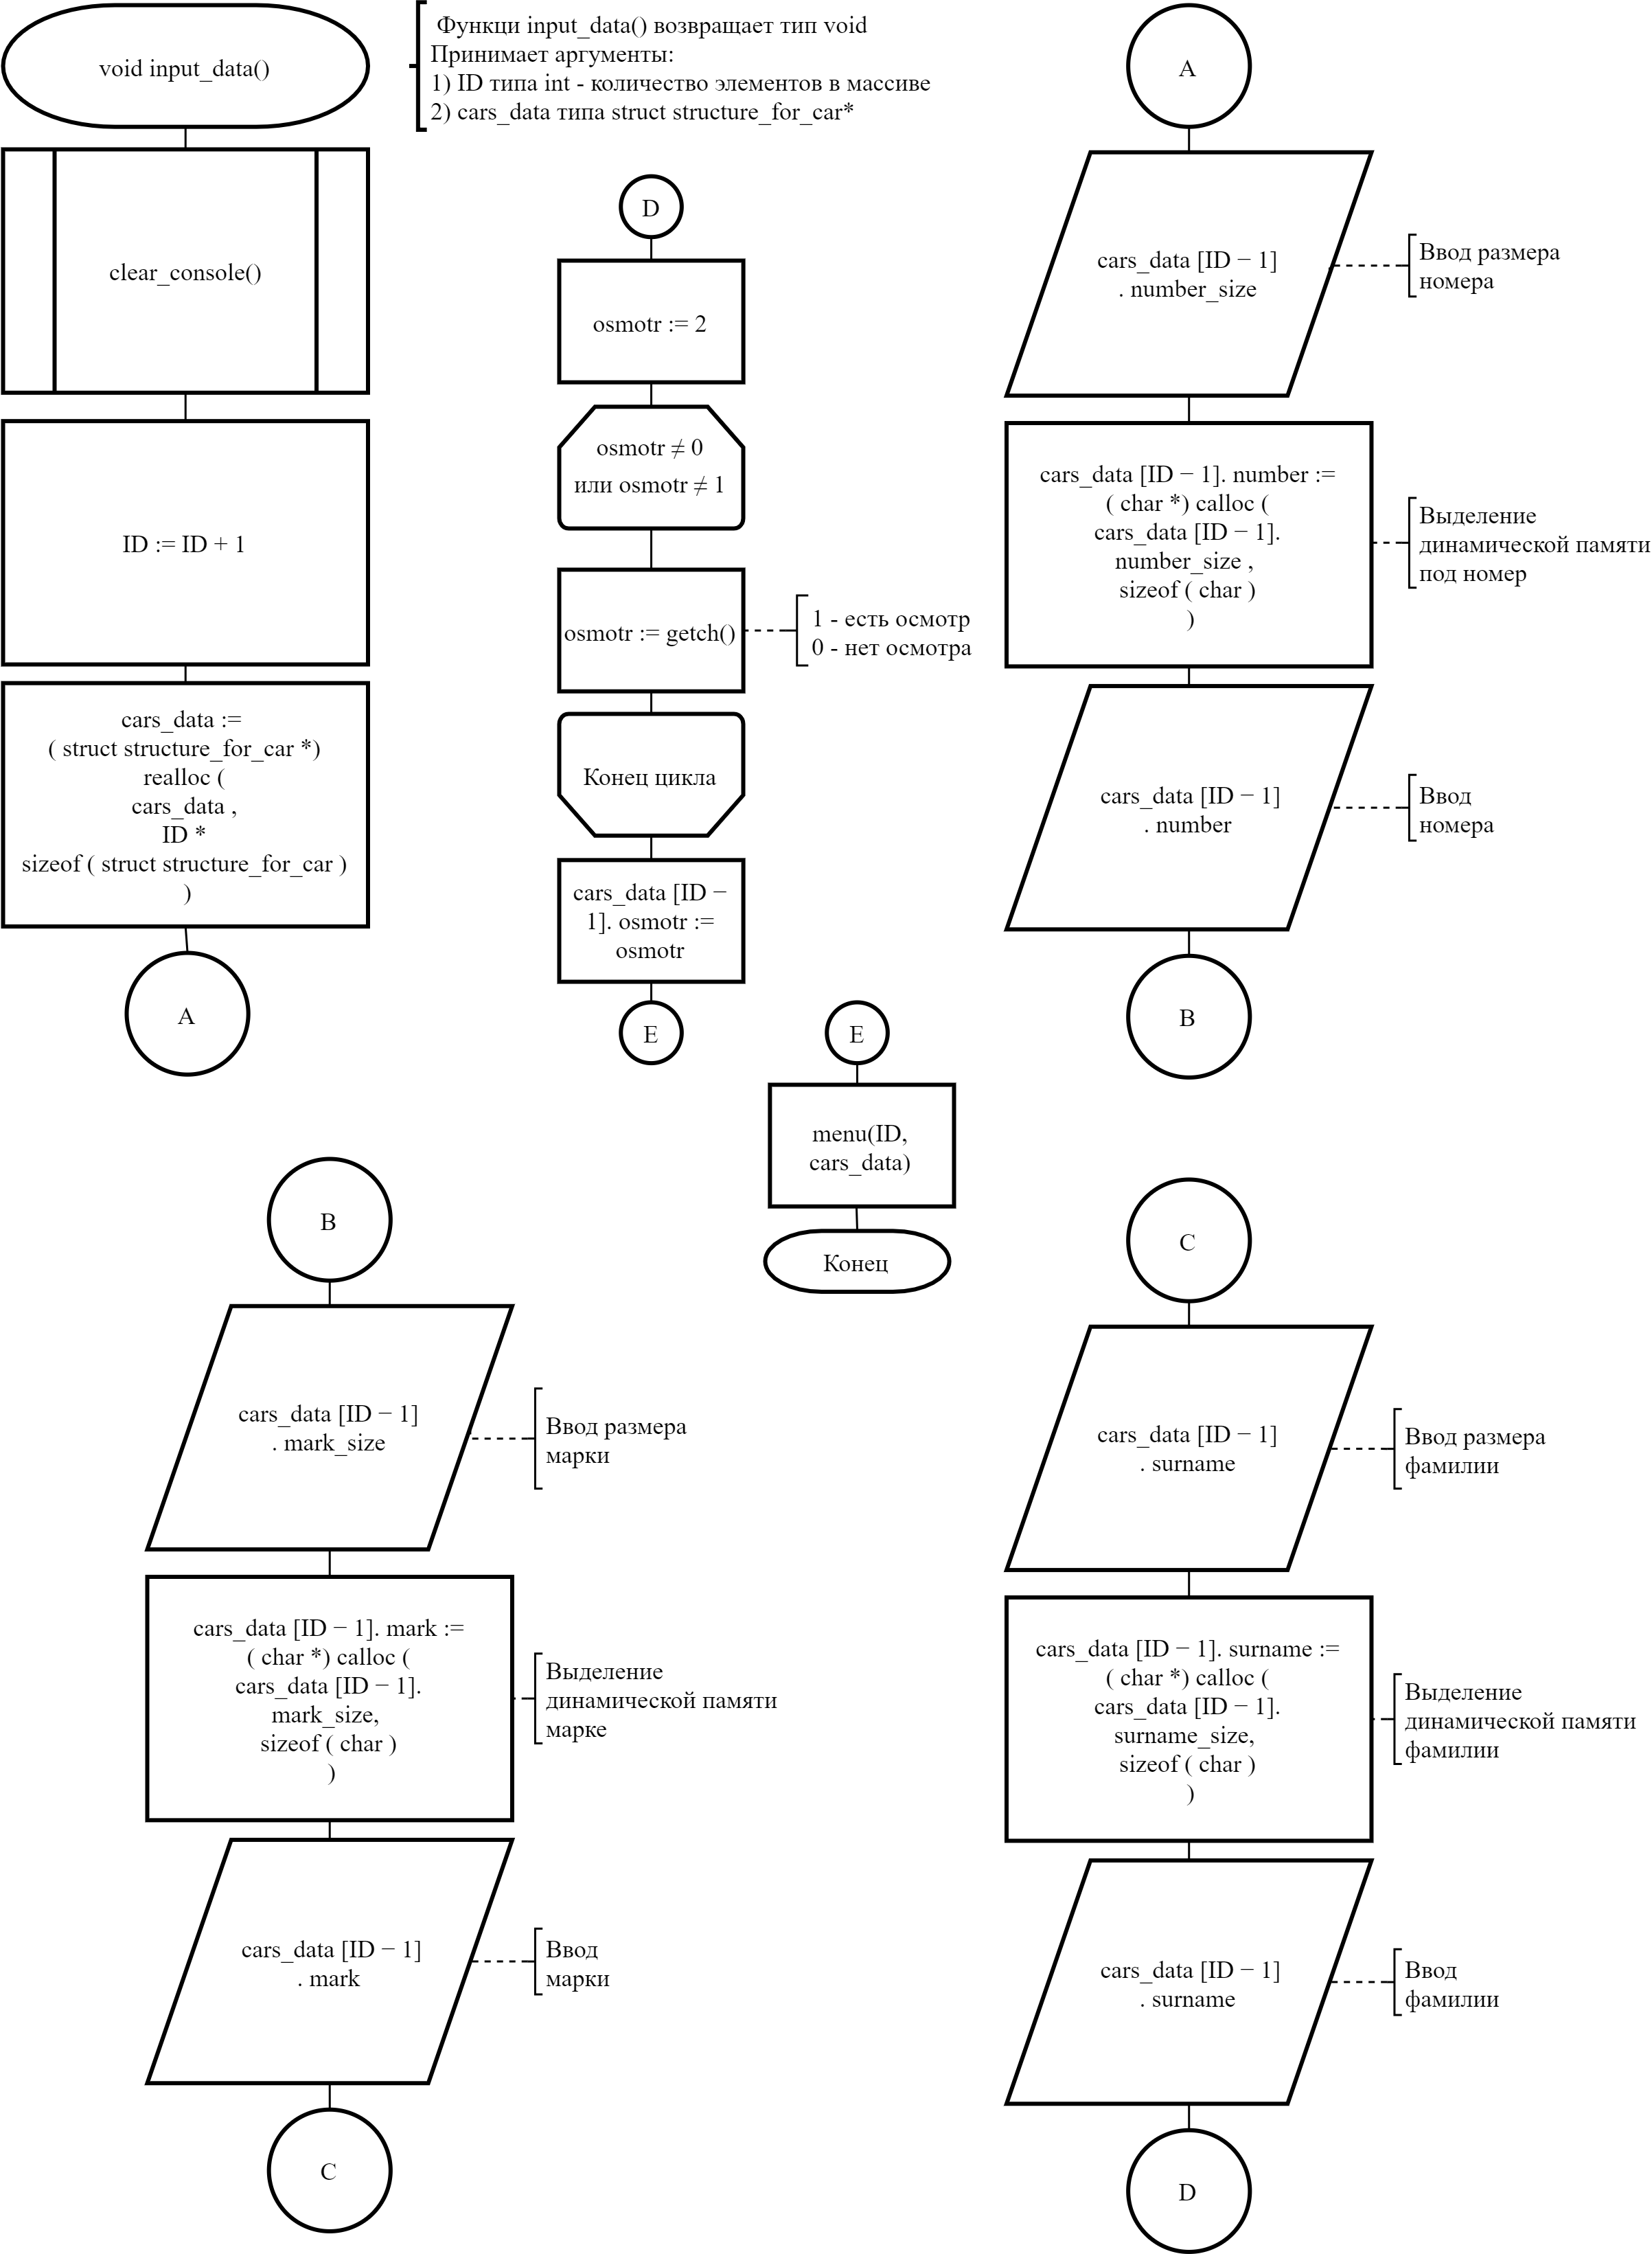
\includegraphics[width=16cm]{13/flowcharts/input_data.png}
    }
    \caption{input\_data()}
    \label{fig:input_data}
\end{figure}

\begin{figure}[h]
    \center{
        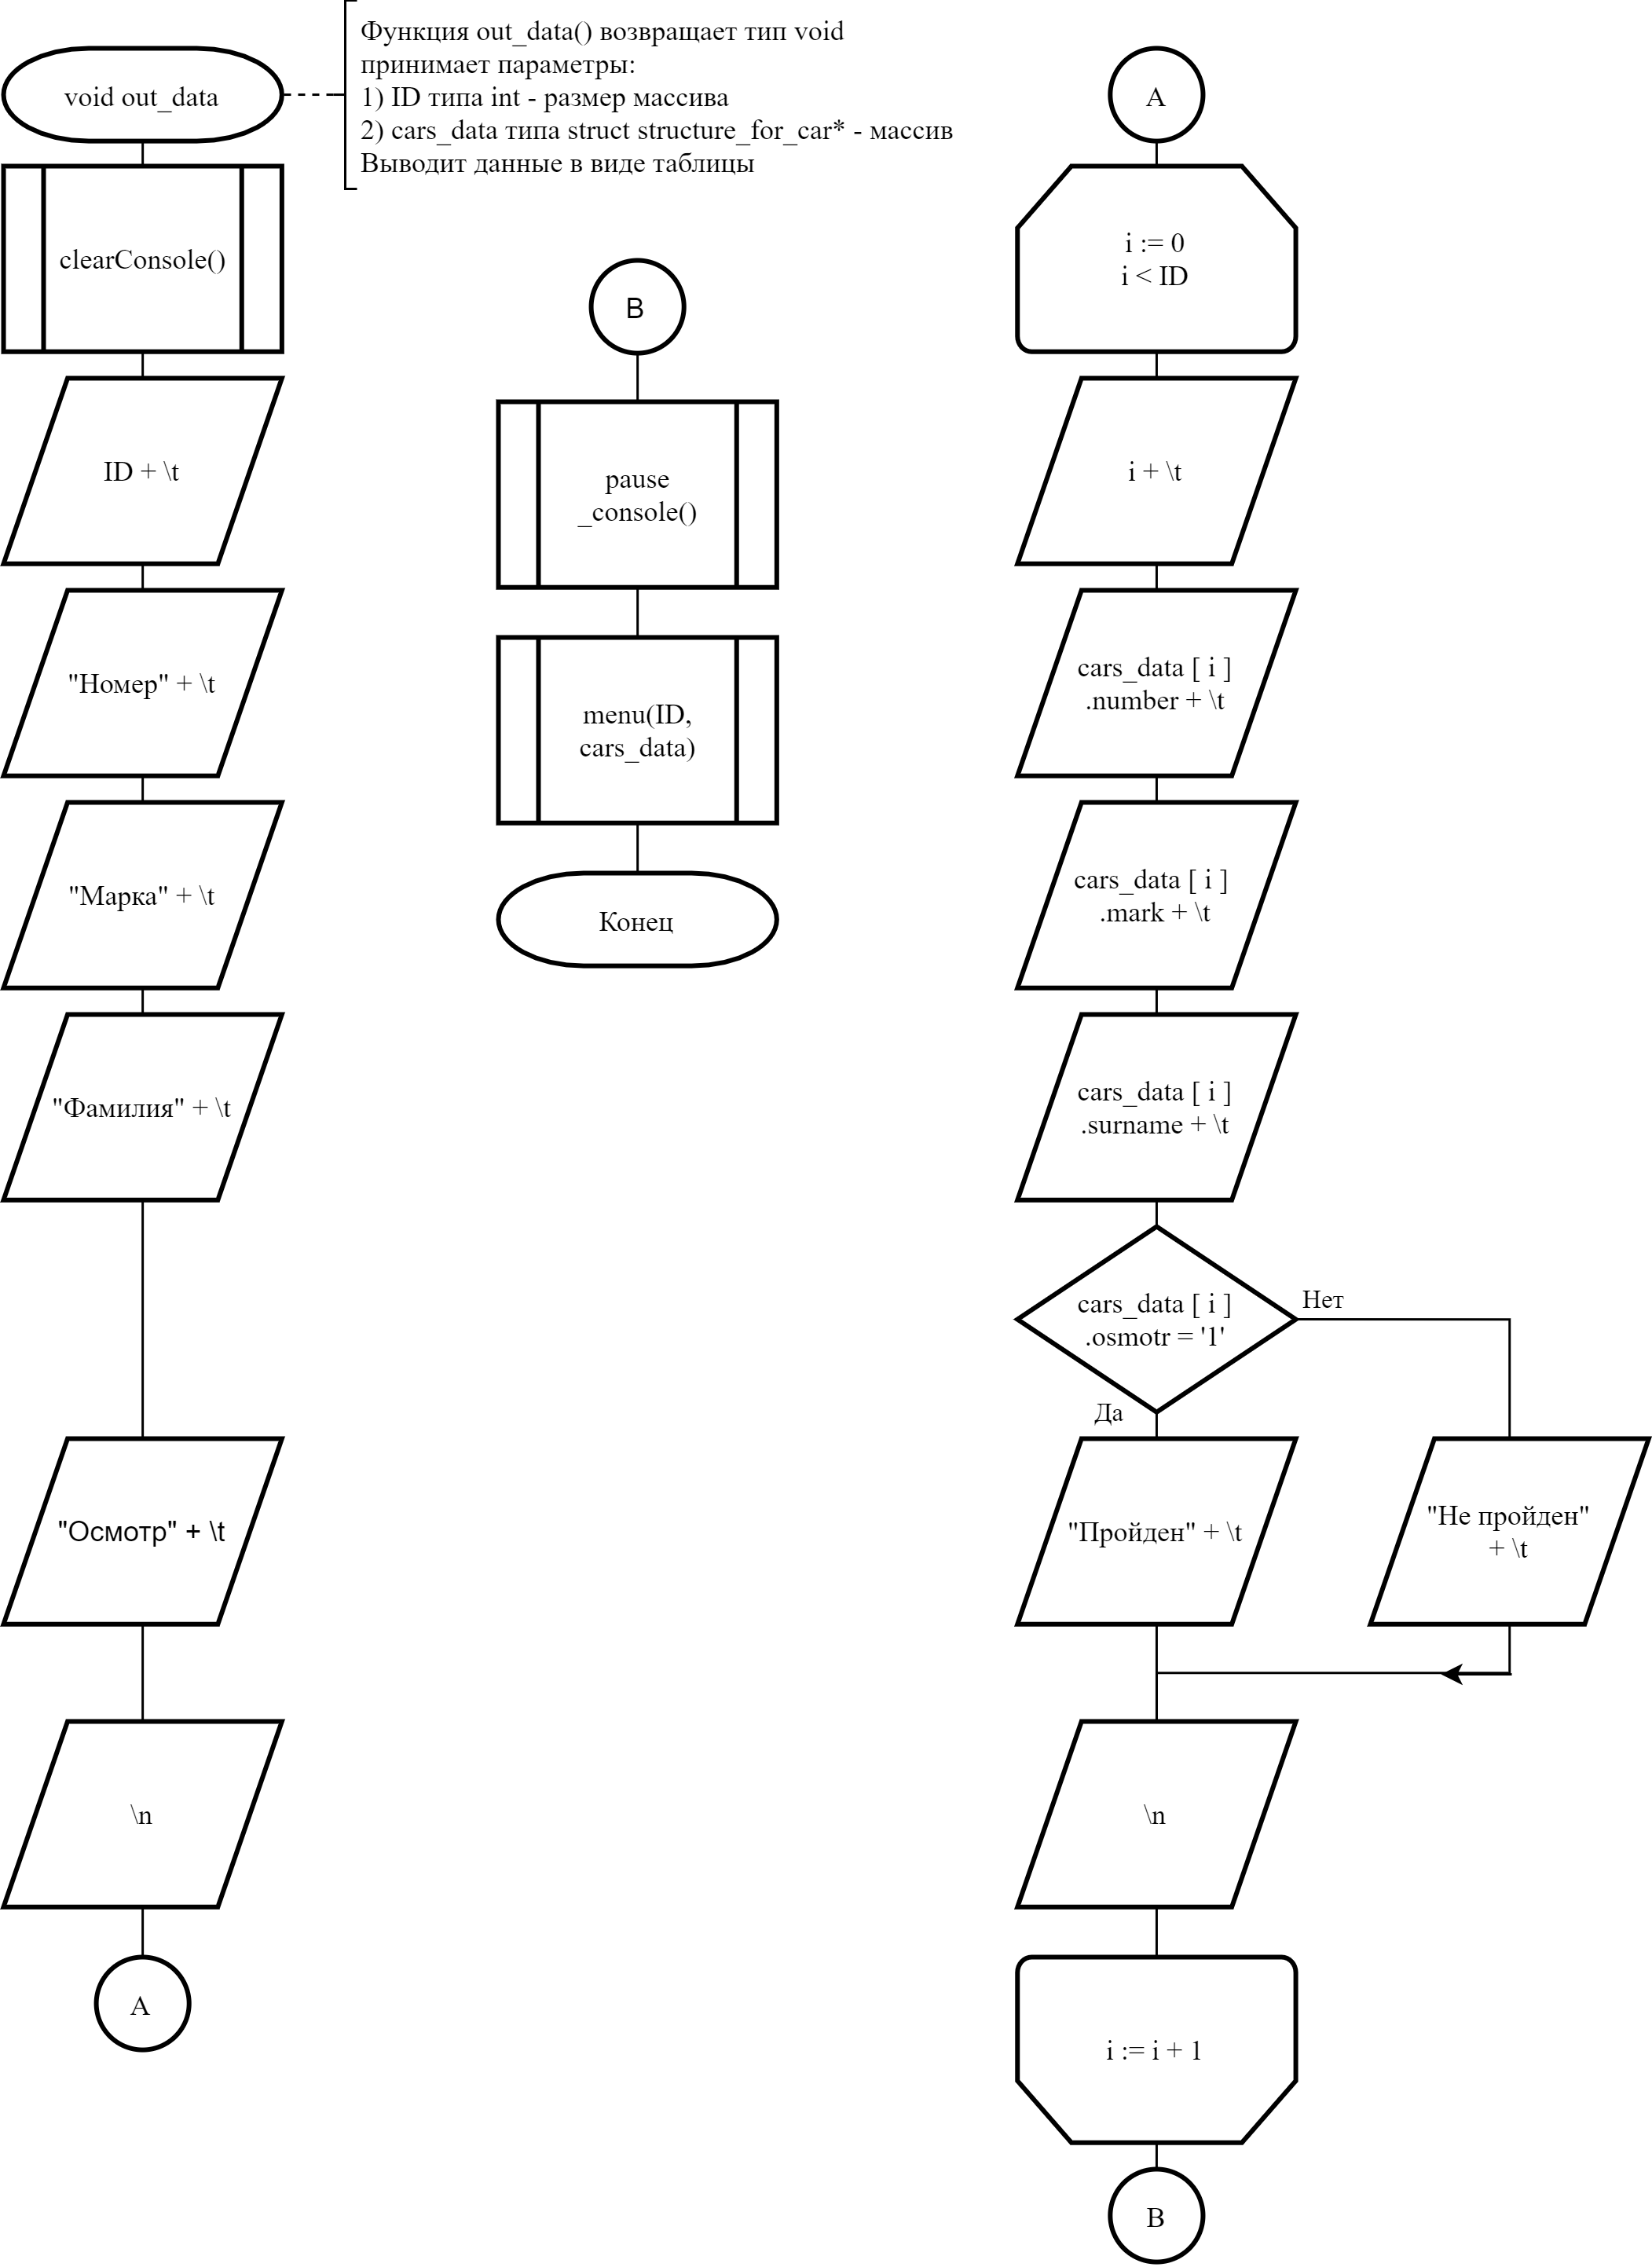
\includegraphics[]{13/flowcharts/out_data.png}
    }
    \caption{out\_data()}
    \label{fig:out_data}
\end{figure}

\begin{figure}[h]
    \center{
        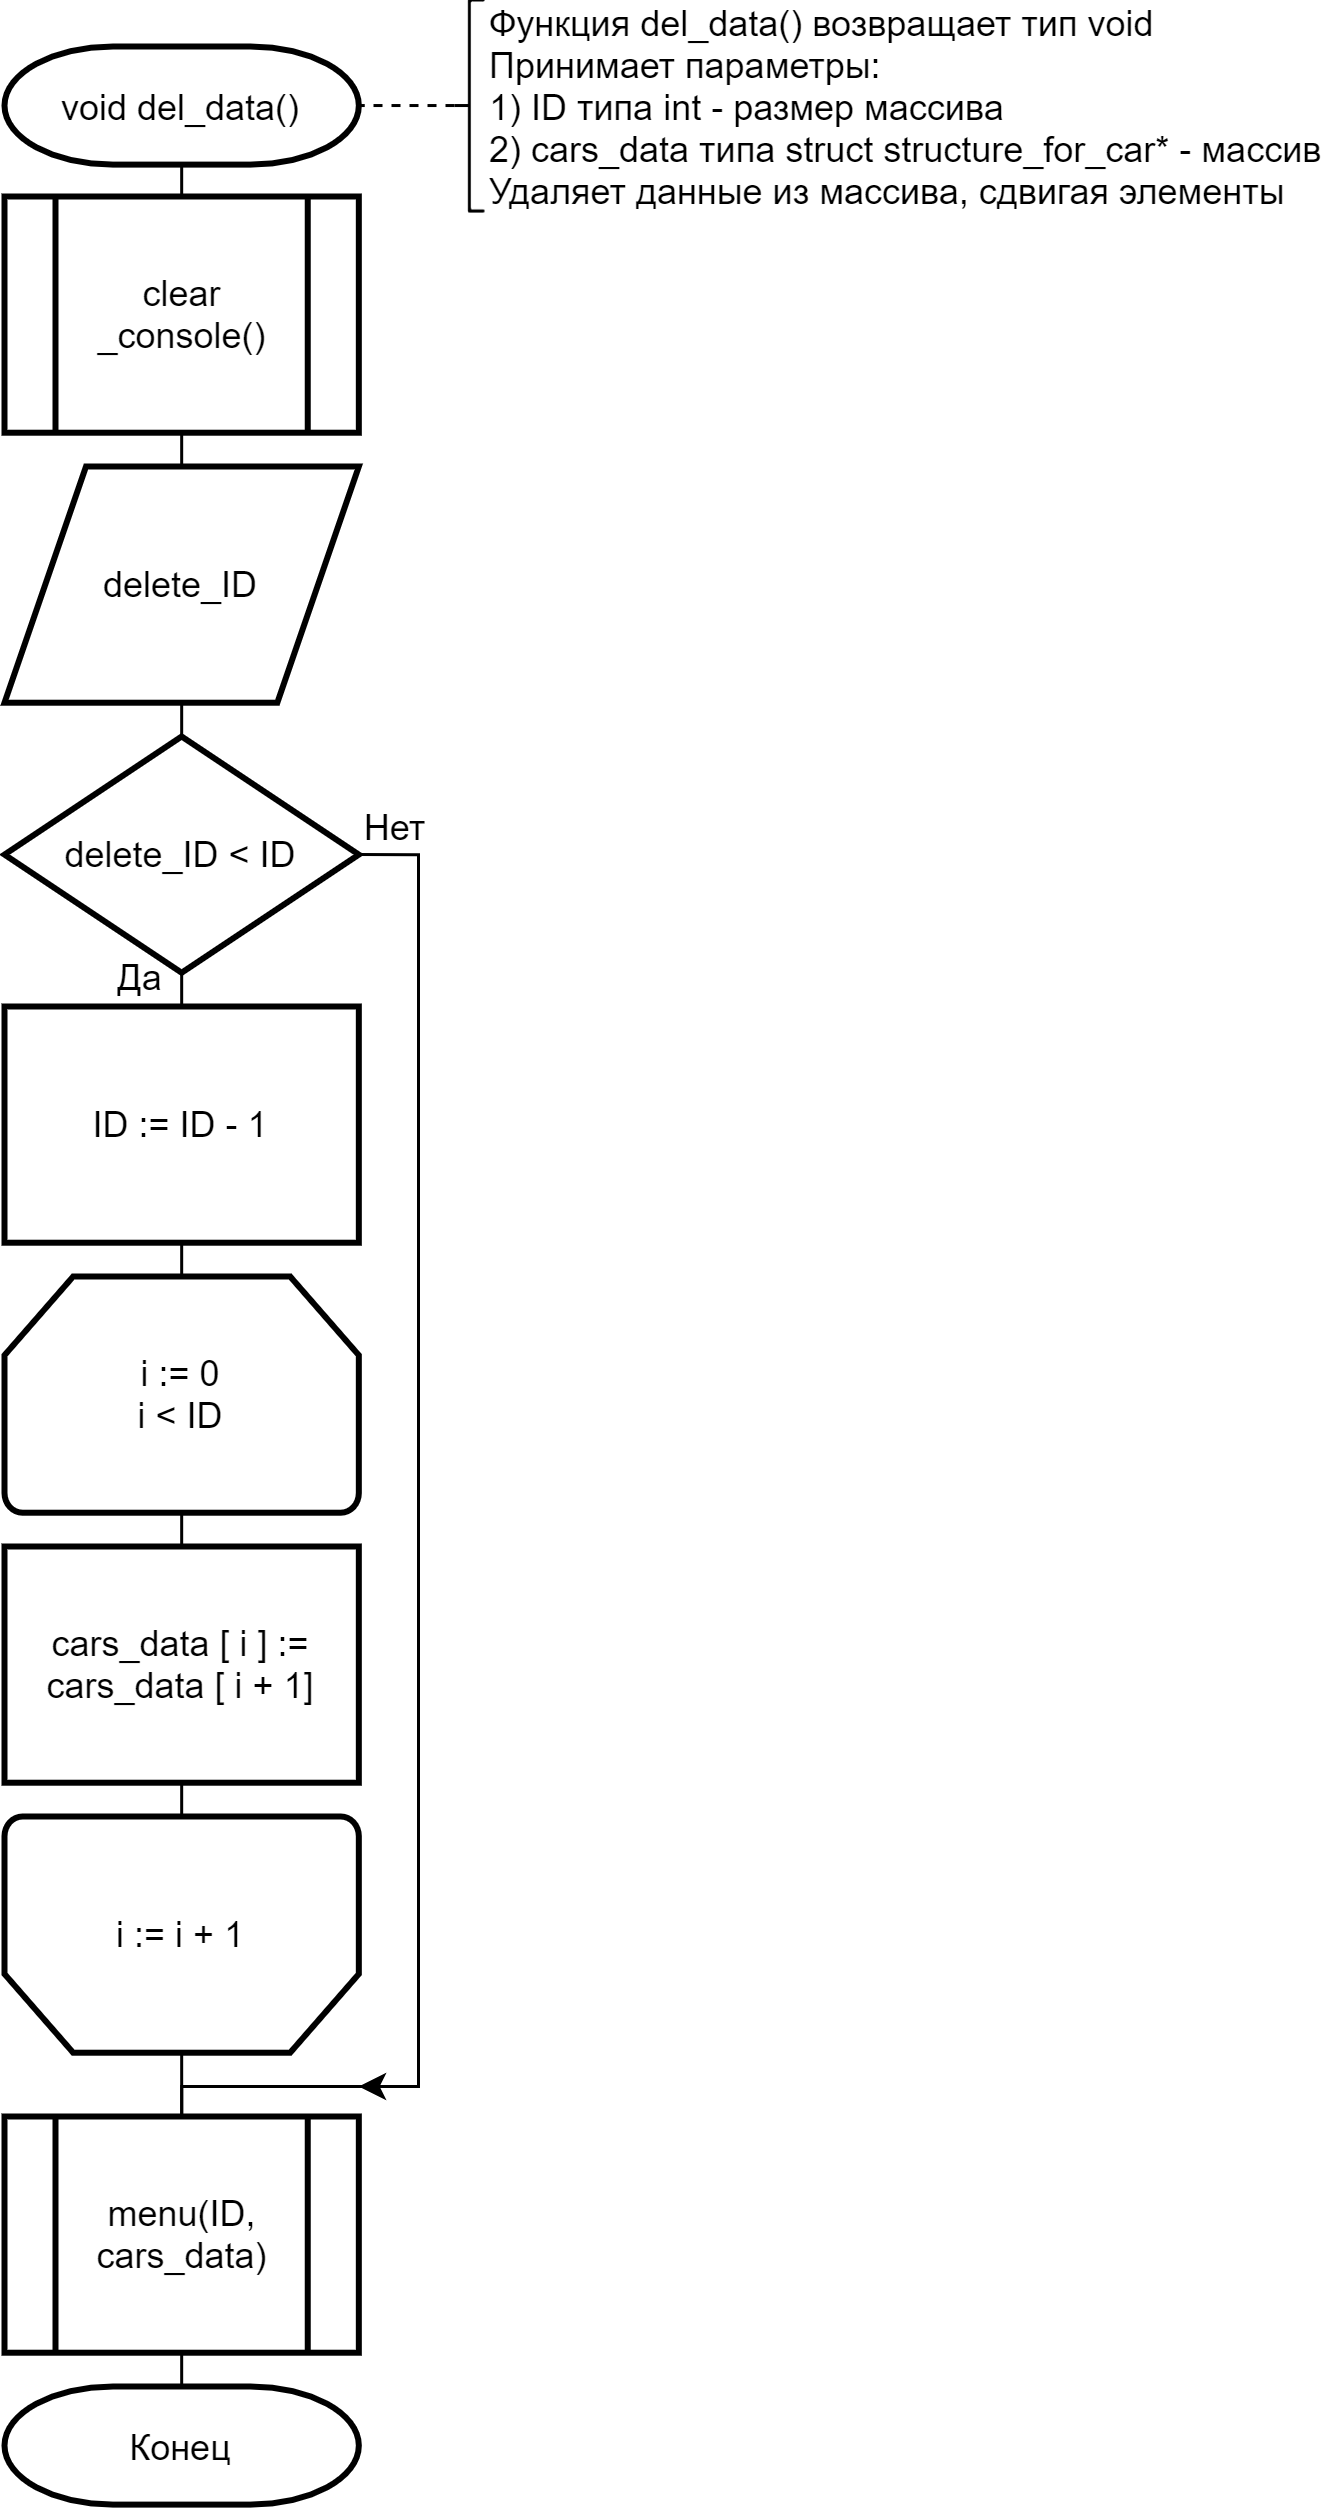
\includegraphics[]{13/flowcharts/del_data.png}
    }
    \caption{del\_data()}
    \label{fig:del_data}
\end{figure}

\end{document}